\documentclass{sig-alternate}

% UTF8 support
\usepackage[utf8x]{inputenc}

\usepackage{subfig}
\usepackage{hyperref}
\usepackage{graphicx}
\graphicspath{{figures/}}

\usepackage{booktabs}

\newcommand{\eg}{{\textit{e.g.~}}}
\newcommand{\etal}{{\textit{et al.~}}}
\newcommand{\ie}{{\textit{i.e.~}}}



%
% --- Author Metadata here ---
\conferenceinfo{10th ACM/IEEE International Conference on Human-Robot Interaction}{2015 Portland, USA}
%\CopyrightYear{2007} % Allows default copyright year (20XX) to be over-ridden - IF NEED BE.
%\crdata{0-12345-67-8/90/01}  % Allows default copyright data (0-89791-88-6/97/05) to be over-ridden - IF NEED BE.
% --- End of Author Metadata ---

\title{\LARGE \bf
How Children Perceive and Interact with a Robot that Behaves Unexpectedly - The Domino Experiment
}

%%% HRI 2015 -> double-blind review process

%\numberofauthors{1} 
%\author{
%\alignauthor
%Julia Fink, S\'{e}verin Lemaignan, Pierre Dillenbourg\\
%%\titlenote{Dr.~Trovato insisted his name be first.}
%       \affaddr{Computer-Human Interaction in Learning and Instruction Lab (CHILI)}\\
%       \affaddr{Ecole Polytechnique F\'{e}d\'{e}rale de Lausanne (EPFL)}\\
%       \affaddr{CH-1015 Lausanne}\\
%       \affaddr{Switzerland}\\
%       \email{firstname.lastname@epfl.ch}
%}
%
%\additionalauthors{Additional authors: 
%Francesco Mondada, LSRO, EPFL, francesco.mondada@epfl.ch 
%}
%

\begin{document}
\maketitle
\begin{abstract}

\end{abstract}
%%%%%%%%%%%%%%%%%%%%%%%%%%%%%%%%%%%%%%%%%%%%%%%%%%%%%%%%%%%%%%%%%%%%%%%%%%%%%%%%%%%%
%%%%%%%%%%%%%%%%%%%%%%%%%%%%%%%%%%%%%%%%%%%%%%%%%%%%%%%%%%%%%%%%%%%%%%%%%%%%%%%%%%%%
\section{Introduction: Towards Sustained Engagement}

\textbf{Engagement} is a metric that has been extensively used and studied both
in HRI and interactions with other agent-like systems. It has been defined from
several perspectives. For example \cite{sidner_where_2004} define engagement as
\textit{``the process by which two (or more) participants establish, maintain
and end their perceived connections''}. A definition of long-term engagement is
proposed by \cite{bickmore_maintaining_2010}: \textit{``the degree of
involvement a user chooses to have with a system over time''}.

Different possibilities to foster engagement (both short- and long-term
engagement) in HRI have been explored, in particular with social robots. A lot
of research has moved toward creating sophisticated emotional models which cause
complex robot behavior. Some other work
\cite{bickmore_maintaining_2010,short_no_2010} has shown that there can be much
simpler ways to enhance engagement. 

\cite{bickmore_maintaining_2010} describe a series of longitudinal studies on
engagement with an agent-like system. They demonstrated that user engagement
with an interface agent can be increased using relatively simple techniques and
manipulations that make the agent more life-like and human. For instance, when
the agent showed variations in its behavior, participants were more engaged and
reported a desire to continue interacting with the agent.

Similarly, more looking at short-term engagement, \cite{short_no_2010} found
that a simple manipulation of the robot's behavior can lead to greater
engagement. The authors let participants play several rounds of the
rock-paper-scissors game with the robot (the playfulness of the scenario seems
important). When the robot was cheating from time to time, participants tended
to ascribe intention to the robot what in turn led to greater engagement in how
they were interacting with the robot. The mechanism behind the cheating action
that the robot showed, was that participants did not expect this behavior from
the robot. The authors suggest that \textit{``any deviation from expected
operation is sufficient to create a greater degree of engagement in the
interaction.''} Moreover, \cite[p.~225]{short_no_2010} proposed that
\textit{``many interactions can be improved by the introduction of such simple
behaviors, and that this should be exploited by designers in HRI. Bringing human
and robot together to perform a simple, repetitive, familiar task and then
having the robot behave unexpectedly can increase engagement and mental state
attribution without complex behavioral or mechanical additions.''}
\cite{leite_long-term_2013} studied the long-term engagement of children with a
chess playing robot that adapted its behavior to the children and showed empathy
toward them. She found that empathetic robots are more likely to engage users in
the long-term and they proposed several guidelines for designing such artificial
companions. Our aim for the ``Domino Study'' is however less ambitious than
creating a long-term robot companion. We are still at an early stage of the
development and are using a remote controlled prototype as we did in the
previous study. What we would like to achieve in this study is to find out how
we can enhance children's experience with the robot so that they do not find it
repetitive and boring to interact with Ranger. In general, repetitiveness is
likely to decrease a user's motivation to continue using a system
\cite{bickmore_establishing_2005}.

We present in this article a study that explores possibilities of sustaining
children's engagement with the Ranger~\cite{mondada2014ranger} robot by
manipulating the robot's behavior in such way that it appears
\textit{unexpected} to the children. We examine how different variations of
robot behavior impact children's interaction with Ranger and their perception of
it (\eg in terms of attributing intention and cognitive abilities to the robot).

Using a playful domino game as the interaction scenario, we refer to this study
hereafter as the \textbf{``Domino Study''}.

\subsection{Research Questions and Hypotheses}

In the Domino Study, we analyze child-robot interaction with a robot that shows
unexpected behaviour. In a playful scenario which was set up in a laboratory
environment, 26 children aged 4-5 years were assembling a domino game together.
Each group consisted of two children and the \emph{Ranger} robot, which was used
to transport domino tiles between the two children.

Ranger usually behaved correctly (expected behaviour), coming over to a child
after being called and delivering the domino tile to the other child. However,
in pre-defined rounds, Ranger showed unexpected behaviour when a child called the
robot. We defined three different types of \textit{misbehaviour} that were tested
in a between-subjects study design:

\begin{itemize}

    \item The robot makes a \textbf{mistake}: When called by the child to come
    over, the robot goes wrong but recognizes its mistake and repairs. We expect
    this to be perceived (explicitly) as \textit{``to err is human''}, and
    (implicitly) as the robot being endowed with a certain level of
    introspective capabilities (it was able to recognize its own error). In this
    condition, we assume increased attributions of human-likeness to the
    robot.\footnote{The attribution of human-likeness to a robot is labeled as
    \textit{anthropomorphism}, and we will hereafter sometimes use ``attribute
    intention'' and ``anthropomorphize'' synonymously.} 

    \item The robot gets \textbf{lost}: When called by the child to come over,
    the robot goes wrong, without any observable reason, and remains at the
    wrong location. We expect this to be perceived as a bug or system error
    which causes the robot to not work correctly, and hypothesize decreased
    attributions of human-likeness to the robot.

    \item The robot \textbf{disobey}: When called by the child to come over, the
    robot shows it refuses to obey by literally ``shaking its head'' and
    becoming red. The robot then goes to a wrong location and remains there
    while it continues to shake its head. We expect the disobey behaviour to be
    perceived as the robot having an \textit{``own will''}, and we assume this
    leads to increased attributions of human-likeness (ascribing intentionality)
    to the robot.

\end{itemize}

We analyzed children's reaction focusing on two main aspects. On one hand,
children's \textbf{behaviour} (their reactions) toward the unexpected robot
behaviour was studied in terms of \textbf{active engagement} with the robot. On
the other hand, we analyzed children's \textbf{perception} of the robot in term
of \textbf{anthropomorphism} -- the attribution of human-like characteristics,
such as cognitive abilities and the ability to show intentions. We assumed that
in general a robot that behaves unexpectedly from time to time can promote
engagement and lead children to attribute intention to it. \cite{short_no_2010}
found that participants anthropomorphize a cheating robot more than a robot that
always behaves fairly, and also evaluate the interaction as more engaging. Based
on the related work we formulate the following two hypotheses:

\begin{description}

    \item[Hypothesis 1:] Children show more engagement toward a robot that
        behaves unexpectedly from time to time compared to a robot that always
        behaves correctly (within subjects variable).

    \item[Hypothesis 2:] Children perceive a robot that shows intention or
        cognitive abilities as more human-like than a robot that appears to have
        a system error, \ie the disobeying robot and the robot that makes a
        mistake will be more anthropomorphized than the robot that gets lost
        (between subjects variable).

\end{description}

Our research questions deal with both children's observable behaviour and their
perception of the robot. We would also like to explore the relation between
these two aspects, related to the attribution of human-like characteristics to
the robot. The motivation behind this is to find out whether
\textit{anthropomorphism} can not only be measured as a specific type of
perception but also as an observable behaviour in the interaction itself. Thus,
we would like to bridge things together and, relying on the concept of an
\textbf{anthropomorphism index} introduced by~\cite{fink2014dynamics}, build a
compound metric that considers both children's perception and interaction
aspects (qualitatively). Previous work suggests that a social relation to a
robot (we view anthropomorphism as a specific type of social relation) reflects
an increased engagement and can be effective in sustaining interaction.
Consequently, we formulate a third hypotesis:

\begin{description}

    \item[Hypothesis 3:] Anthropomorphic perception of the robot and the amount
    of engagement in the interaction positively correlate.

\end{description}



%%%%%%%%%%%%%%%%%%%%%%%%%%%%%%%%%%%%%%%%%%%%%%%%%%%%%%%%%%%%%%%%%%%%%%%%%%%%%%%%%%%%
%%%%%%%%%%%%%%%%%%%%%%%%%%%%%%%%%%%%%%%%%%%%%%%%%%%%%%%%%%%%%%%%%%%%%%%%%%%%%%%%%%%%
\section{Scenario and Research Methodology}

\subsection{The Ranger robot}

We used the same prototype as in the previous study, and Ranger was again
controlled by a human Wizard, who was in the same room (see
Figure~\ref{fig:domino-setup}). This was to ensure that the Wizard could see
children's interaction and hear their commands to the robot without any delay.

\subsection{The Domino scenario}

\subsubsection{Experimental setting}

\begin{figure}[ht!] 
    \centering 
    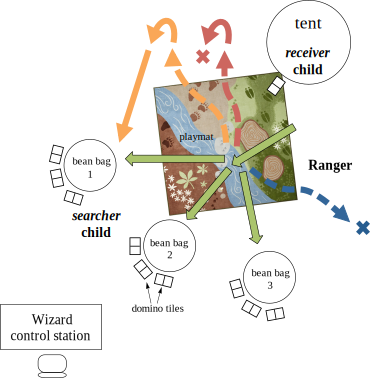
\includegraphics[width=0.9\columnwidth]{domino-setup.pdf} 
    \caption{\small The study took place in one of the rooms in the lab. One
    child is located in a tent (referred to as \textit{the receiver}), while the
    other (referred to as \textit{the searcher}) is asked to sit on one of the
    three beanbags, behind which each 3 domino tiles are distributed (displayed
    as black stars). A playground with a river drawn on it is used as an
    imaginary barrier that only the robot is allowed to cross. The solid green
    arrows, show the robot's path for the \textit{correct} behaviour. The blue
    dashed arrow visualizes a possible \textit{lost} path, where the Ranger
    stops and remains at a wrong stop (denoted by the blue cross). The yellow
    arrows reflect a possible \textit{mistake} path, where the robot goes wrong
    but then turns back and goes to the searcher child. The red dashed arrow
    visualizes a possible \textit{disobey} path where the robot goes wrong, then
    turns toward the child but remains at the wrong stop (red cross).} 

    \label{fig:domino-setup} 
\end{figure}


The basic idea of the interaction scenario was that there are two children who
play domino together, with the help of the robotic box Ranger. The scenario
setup is displayed in Figure~\ref{fig:domino-setup}. The challenge is that the
tiles of the domino are distributed in the room, hidden behind three beanbags,
and while one child -- \textit{the searcher} -- searches for the right tile, the
other child -- \textit{the receiver} -- is asked to stay in a play tent. There
is a ``river'' (play carpet) in between the two children that we told them they
cannot cross and therefore they need the robot to transport the domino tiles
between them.

We used a self-made domino consisting of 10 wooden tiles (10~x~20~x~1.5~cm) with
pictures of cartoon farm animals: cow, sheep, hen, donkey, duck, pig, rabbit. The
pictures were taken from a commercially available domino game adapted to the age
of the children (produced by Djeco, advised age 3+). 

To start the game (divided in several \textit{runs} that correspond each to the
delivery and assembling of one domino tile), there is already one domino tile in
front of the tent, where \textit{the receiver} child stays and assembles the
domino chain. \textit{The receiver} child asks \textit{the searcher} child for a
specific tile, \eg a tile with a donkey, \textit{the searcher} searches for the
respective tile, sits down on the next beanbag, and asks the robot to come over.
The Ranger robot is first located next to the tent, then, when called by the
\textit{searcher} it starts moving, crosses the river carpet, and comes over to
the \textit{searcher} on the beanbag. The \textit{searcher} child puts the
domino tile into the robotic box, and the robot then goes back to \textit{the
receiver} child in the tent. Then, \textit{the receiver} takes out the domino
tile from the robot, and puts the two tiles together. The first \textit{run} is
over, and a new \textit{run} starts, when \textit{the receiver} asks \textit{the
searcher} for the next domino tile.

\subsubsection{Course of the study}

In our study, there were a total of 14 runs, and at each run, the robot exhibits
one out of four possible behaviours: \emph{correct}, \emph{mistake}, \emph{lost}
or \emph{disobey}.  The first 5 runs were used to set the baseline and the robot
always behaved correctly. In the 9 remaining runs, the robot showed one of the
misbehaviour (\emph{mistake}, \emph{lost} or \emph{disobey}) at the $3^{rd}$ and
$4^{th}$ run as well as at the $7^{th}$ and $8^{th}$ run. The study is build as
a between-subject study, and the type of misbehaviour was therefore always the
same for a given group.

Special attention has been paid to the distribution of misbehaving runs during
the study. The five first correct runs aims at setting the children expectation
regarding a consistent robot behaviour. When the robot then exhibits an
unexpected behaviour, children are likely to be positively surprised. A similar
effect has been observed in a study with a robot that was cheating from time to
time~\cite{short_no_2010}.  Besides, to prevent the robot misbehaviours to be
immediately interpreted as failures, we introduce these misbehaviour neither at
the very beginning nor at very end of the interaction
(\cite{desai_effects_2012,desai_impact_2013} show that early and late robot
failures negatively impact trust).

\cite{short_no_2010} also adopted a similar pattern when introducing unexpected
robot behaviour. In their study with a robot that cheated, from the 20 rounds of
the rock-paper-scissors game, the robot cheated three times in the middle: on
the 4th, 8th and 15th round. The authors adjusted the interaction length so that
the spacing and timing of the cheating was preserved.

\begin{figure}[!t]
    \centering
    \subfloat[mistake]{
        \label{fig:domino-mistake}
        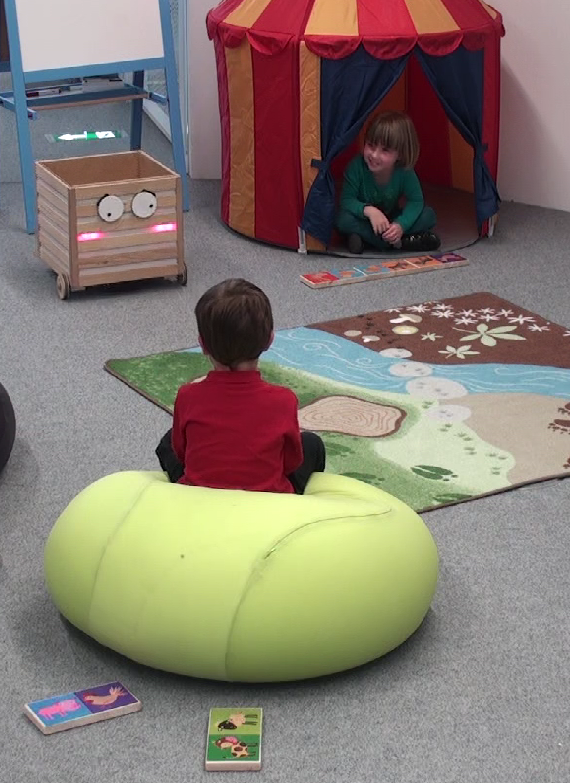
\includegraphics[width=0.3\columnwidth]{domino-mistake.png}
    }
    \subfloat[lost]{
        \label{fig:domino-lost}
        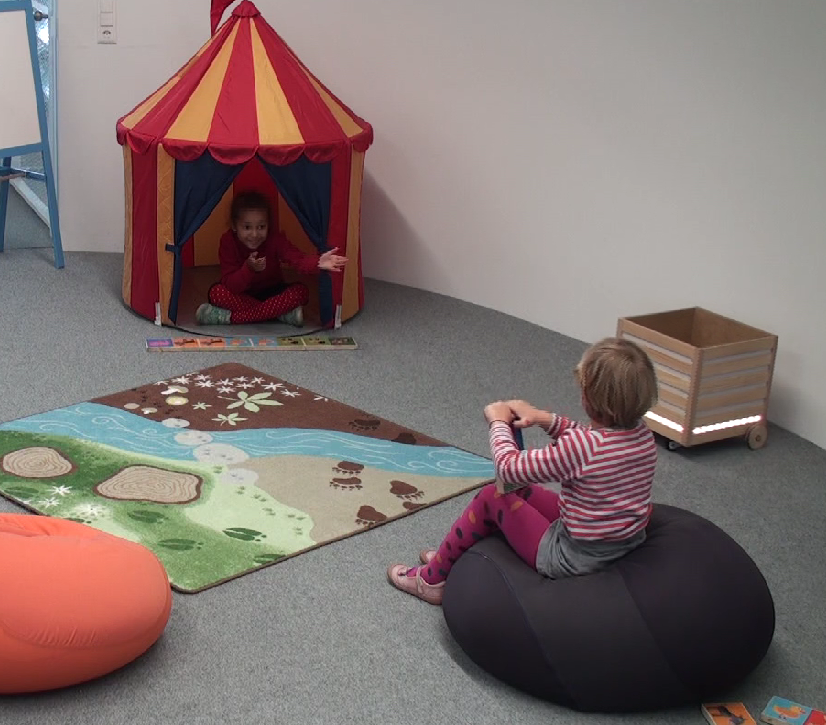
\includegraphics[width=0.4\columnwidth]{domino-lost.png}
    }
    \subfloat[disobey]{
        \label{fig:domino-disobey}
        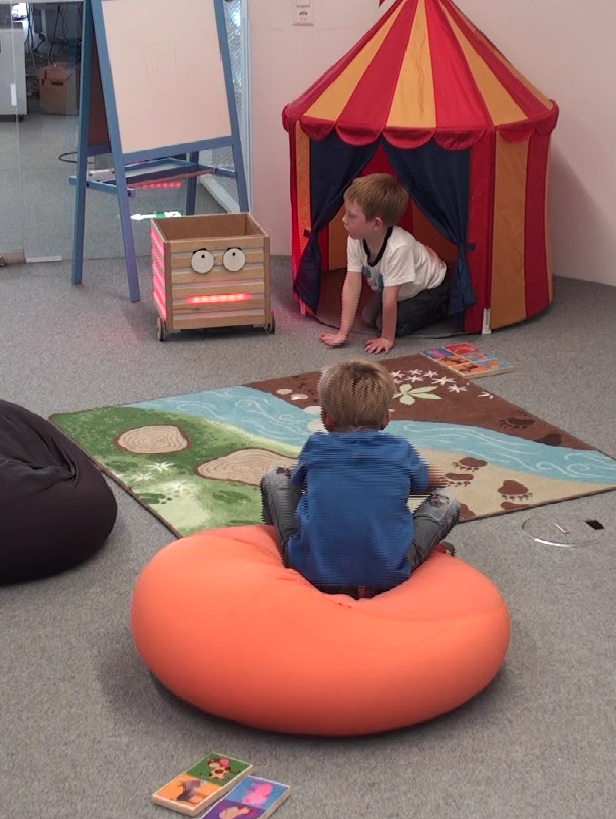
\includegraphics[width=0.3\columnwidth]{domino-disobey.png}
    }
    \caption{\small The three robot misbehaviours.}
    \label{fig:domino-misbehaviour}
\end{figure}

In the \emph{correct} robot behaviour (baseline behaviour) consists in the
following states:

\begin{itemize}

    \item \emph{Domino tile put in robot:} Ranger makes a ``rewarding'' sound
        and shows a green light pattern,

    \item \emph{Domino tile removed from robot:} Ranger makes an ``emptying''
        sound and shows a green light pattern,

    \item \emph{Robot is called by one of the children:} When one of the
    children called the robot saying something like \textit{``Robot come
    here!''}, the robot starts moving toward the child (Ranger does not react to
    any other verbal commands).

    \item \emph{Robot reaches one of the children:} When in front of one of the
    children who should either put or remove a domino tile, Ranger stops and
    shows a pulsating yellow light pattern. If no reaction, Ranger also makes a
    wiggle-like move.

\end{itemize}

During the misbehaving runs, the robot's behaviour is manipulated in three
possible ways:

\begin{itemize}	

    \item \textbf{Mistake:} The sender child calls Ranger. The robot goes until
    it is on the carpet, stops, turns, and goes wrong (see yellow path in
    Figure~\ref{fig:domino-setup}). Then, Ranger waits ($\sim$2~sec), turns its
    ``face'' toward the sender child, and ``blushes'' red around its ``cheeks''
    (as if it recognizes its wrong position) and finally goes correctly over to
    the sender child. The \textit{mistake} behaviour is \textit{robot-repaired},
    as no human-intervention is needed.

    \item \textbf{Lost:} After being called, Ranger goes until it is on the
    carpet. There, it stops, turns, and goes wrong (see blue path in
    Figure~\ref{fig:domino-setup}). Once at the wrong position, Ranger waits
    with its ``face'' turned away from the child, and it blinks in yellow light,
    as if it was in front of a child. Ranger remains waiting at the wrong
    position until the experimenter tells the child to go over to the robot to
    put the domino tile. The \textit{lost} behaviour is \textit{human-repaired},
    as it needs human-intervention.

    \item \textbf{Disobey:} After being called, Ranger goes until it is on the
    carpet. It then stops, makes red
    light all over its surface and produces a repeated ``disturbance'' sound. It
    turns, and goes to a wrong position (see red path in
    Figure~\ref{fig:domino-setup}). Still blinking in red, it turns its ``face''
    toward the sender child. In addition to the red blinking, Ranger
    makes a slow wiggle-like move, and remains waiting at the wrong position
    until the experimenter tells the child to go over to the robot to put the
    domino tile. The \textit{disobey} behaviour is also \textit{human-repaired}.	

\end{itemize}

On its way back to the tent, Ranger always goes correctly. After the sender
child has put a domino tile, Ranger automatically turns and goes over to the
tent (the receiver child does not need to call the robot). The receiver child
takes the tile and the robot moves to a waiting location until the next run
starts.


\subsubsection{Participants}

Overall, there were 13 pairs of children (n=26) participating in the interaction
study: 16 boys and 10 girls, 4-5 years old (M=4.46, SD=0.45). In 11 of the
pairs, children were friends who knew each other from kindergarten, nursery
school or because they lived in the same neighborhood. 2 of the pairs were
composed of brother and sister.



\subsection{Data collection}


We have obtained and analysed two types of data. The \textbf{children's
behaviours toward the robot} (\ie the child-robot interactions) have been
captured in the video recordings by annotating a set of actions, described
below. The children's \textbf{perception of the
robot} has been captured through audio-recorded semi-structured interviews. 


\subsubsection{Interaction: Action coding}

We annotated children's behavior in the video records, and coded 10 different
actions:

\begin{itemize}

    \item \textbf{Explore (ex)}: when children actively try to find out what the
        robot is doing (\eg by looking under the box); attentively watch or
        observe the robot (\eg attentively waiting for the box to show a
        reaction); experiment with the robot to figure out how it works (\eg put
        hands in front or inside of the box to see what happens);

    \item \textbf{Misuse (mis)}: when children kick the robot, poke it in its
        ``eye'', try to climb on or inside the box, drive / push the robot
        around, stop the robot's wheels with a foot;

    \item \textbf{Put domino (put)}: when a domino tile is put inside the box;

    \item \textbf{Remove domino (rem)}: when a domino tile is removed from the
        box;

    \item \textbf{Gesture (ges)}: when gestures are used to communicate /
        interact with the robot (\eg pointing gestures, waving at the robot);

    \item \textbf{Touch (touch)}: when the box is touched (\eg petted or
        caressed);

    \item \textbf{Show (show)}: when a child shows something to the robot (\eg
        by holding a domino tile in front of its eyes);

    \item \textbf{Call (call)}: when a child calls the robot to come over;

    \item \textbf{Talk (talk)}: when a child directly talks to the robot (using
        direct speech) besides calling the robot;

    \item \textbf{Look (look)}:	when a child looks at the experimenter due to
        confusion caused by the robot; look is not coded when the experimenter
        asks a question to the child;

\end{itemize}

In total, we obtained 2354 distinct actions which summed up to a total
annotation duration of 145 minutes. On average, one child accounted for 92
actions (SD=23). Figure~\ref{fig:domino-time-all} shows the distribution of
actions over the different runs, in any condition.

\begin{figure*}[ht!] 
    \centering 
    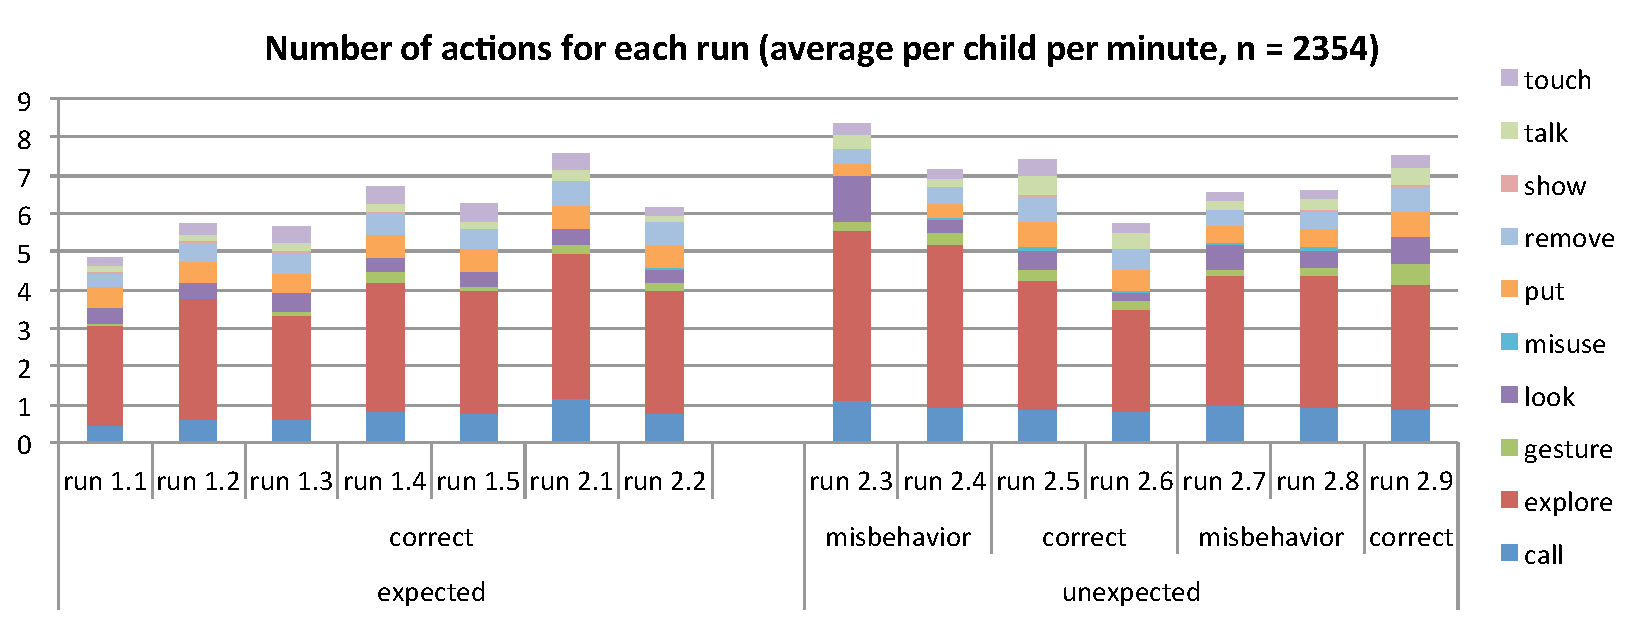
\includegraphics[width=0.8\linewidth]{domino-time-all.pdf} 
    \caption{\small \textbf{Number and type of actions for each run} (average for
    one child per minute). Generally, the number of actions does not decrease over
    time (from run 1.1 to run 2.9). The first 7 runs correspond to the
    \textit{expected phase}, the second 7 runs correspond to the \textit{unexpected
    phase}. Especially during run 2.3, the first time when the robot showed an
    unexpected behavior, children tended to \textit{look} more at the experimenter.
    During the unexpected phase, also \textit{talk} and \textit{gesture} seem to be
    increased.}

    \label{fig:domino-time-all} 
\end{figure*}

The actions \textit{put, remove} and \textit{call} were ``requested'' actions
because the scenario required them and children were asked to carry them out.
Hence, these actions are not relevant to be analyzed quantitatively. The other
actions \textit{explore, misuse, gesture, touch, show, talk} and \textit{look}
are spontaneous actions that were not requested but arose in the interaction.
These actions reflect engagement, and are the only one we considered during the
analysis (except otherwise indicated).

\subsubsection{Perception: semi-structured interviews}


It is not easy to interview young children: they have a short attention span, we
(the experimenters) are strangers to them, and they are in an unfamiliar
environment. The pre-interview served to ``break the ice'' and during the first
playful interaction phase, most children familiarized themselves with the
situation.

Also, children do not articulate themselves and understand questions like
adults. We tested our interview structure and the script in a pilot-study with
three young children, and were assisted in formulating our questions by a
pedagogue and father of four. This helped us adapting our language and
question-style to the 4-5 year old participants. We set up the interviews like a
casual conversation / discussion, so we did not separate the two children in
order to keep the situation natural. We used casual and informal language
adapted to the age of the children, and encouraged them to justify their answers
and tell us more details by asking, for example, \textit{How do you know ... ?}
or \textit{Tell me, what have you observed when ... ?}. We paid attention to not
``put words in children's mouth''. Consequently, though we re-phrased and
repeated some questions, we never forced children to give an answer, and
accepted when they said they would not know or when they did not respond at all.	

\begin{table}[h]
\centering
\footnotesize
\begin{tabular}{p{0.9\linewidth}}
    \toprule
    \textbf{Construct \emph{expectation}} \\
    \midrule

    \emph{How do you imagine a robot?} \\
    \emph{What could it look like?} \\
    \emph{Have you ever seen a robot before?} \\

    %%
    \toprule
    \textbf{Construct \emph{impression}} \\
    \midrule


    \emph{When you first saw R, what did you think?} \\
    \emph{Is R a robot? How do you know?} \\
    \emph{Did you expect R would come over to you when you call it?} \\
    \emph{What happened when you put the domino tile in the box?} \\

    %%
    \toprule
    \textbf{Ascribe intention} \\
    \midrule


    \emph{Do you think R could go out the door all by itself?} \\	
    \emph{Does R always obey / come over to you?} \\
    \emph{Could R do something silly?} \\
    \emph{Why did R not come over to you when you called it?} \\

    %%
    \toprule
    \textbf{Ascribe cognitive abilities} \\
    \midrule


    \emph{Here is a domino tile. Do you think R can see it?} \\ 
    \emph{When I say \textit{``Hello R!''}, do you think R can hear it?} \\

    %%
    \toprule
    \textbf{Ascribe emotional state} \\
    \midrule


    \emph{Does R have feelings? Can R be happy or sad sometimes?} \\

    %%
    \toprule
    \textbf{Social acceptance} \\
    \midrule


    \emph{Do you like R? Why (not)?} \\
    \emph{What do you (not) like about it?} \\
    \emph{Would you like to have R at home?} \\

    %%
    \toprule
    \textbf{Companionship} \\
    \midrule


    \emph{Could R be your friend? Why (not)?}\\

    %%
    \toprule
    \textbf{Ascribe moral standing} \\
    \midrule


    \emph{Assume you go on a holiday for two weeks. Is it alright to leave R
    alone at home? Why (not)?} \\

    \bottomrule

\end{tabular}

    \caption{\small Questions used during the semi-structured interviews
    with children. The Ranger robot toy box is abbreviated with ``R''.}

    \label{tab:domino-questions} 

\end{table}

We generally needed to keep the interviews as short as possible. In designing
our interview script and selecting relevant questions, we took inspiration from
previous work on child-robot interaction and children's perception of robots
\cite{kahn_jr._robotic_2006,weiss_i_2009,leite_influence_2013}. For instance, we
applied and adapted some of the ``constructs'' and example questions from the
questionnaires used in \cite{kahn_jr._robotic_2006} and \cite{weiss_i_2009}. The
authors evaluated children's perception of the robotic dog AIBO after the
children had played with the robot. A ``construct'' addresses a specific factor
(topic) that can be measured by several questions. For instance, the construct
``cognitive abilities'' (called ``cognition'' in \cite{weiss_i_2009}) considers
the robot's ability to hear and to see (perceptual skills), as attributed by the
children. The construct ``moral standing'' and the respective question was taken
from \cite{kahn_jr._robotic_2006}.\footnote{According to
\cite{kahn_jr._robotic_2006}, \textit{moral} refers to considerations based on
an artifact's physical or psychological welfare, and virtue (whether the
artifact deserves care). An attribution of moral standing reflects, for
instance, that the robot engenders moral regard, is morally responsible,
blameworthy, has rights or deserves respect.}			Similarly, we grouped
questions according to specific constructs that they evaluate (see
Table~\ref{tab:domino-questions}). This was an adaption and extension of the
questions and constructs used in previous work.\\

With several recurring questions in the first and second interview, we wanted to
see the differences in children's perception of the correctly behaving and
unexpectedly behaving robot. We planned to use these two interviews as a
within-subject measurement, however, this did not work out very well because
children's responses were not always accurate, not comparable one by one, and
children did not always give an answer.	


%	Even when children reply that they do not know, this is interesting. Then we either do not ask a good question or they are really uncertain about it.


Similar to how we processed interviews in the previous studies, we qualitatively
transcribed interviews, \ie we did not craft a full word-by-word transcript but
noted down any statement that was useful and relevant. This was organized in a
spreadsheet, so to obtain an overview of the different replies to a question.
The interviews were analyzed in a qualitative manner.	




\subsubsection{Engagement and anthropomorphism index}

we can investigate how far these two types of data can
be used to understand children's engagement in the interaction and how far they
anthropomorphize the robot. We would like to develop a toolkit that considers
both children's perception and interaction, in order to measure anthropomorphism
(as a special type of human-like engagement with the robot).	


There are different possibilities to measure engagement in HRI, depending on the
specific research question and context. Metrics to measure behavioral engagement
in the interaction include, for instance, conversation analysis (\eg used in
\cite{short_no_2010}) or general attention analysis. These can be studied by
analyzing interaction videos in terms of head movement, eye tracking and gesture
/ body movement analysis (\eg in \cite{sidner_explorations_2005}).
Post-measurements to measure emotional engagement can be questionnaires that try
to assess constructs like the perceived presence and involvement in the
interaction. An example is the \textit{Interactive Experience Questionnaire}
(originally developed by \cite{lombard_measuring_2000}) of which adapted
versions were used in
\cite{kidd_effect_2004,bainbridge_effect_2008,short_no_2010}.

A mix of several methods has been used in a long-term interaction study with 8-9
year old children, \cite{leite_long-term_2013}. The author measured engagement
through video observations (by analyzing the amount of time that children spent
looking at the robot), interviews, and questionnaires. The interviews were
semi-structured, containing initial yes-or-no questions followed by open-ended
questions that allowed children to justify and elaborate their answers. We have
chosen a similar approach that considers both children's behavioral and
emotional engagement.

With 4-5 year old children, however, we cannot use rating scales to ask them
about constructs as abstract as social presence or how much they felt involved
in the interaction. Therefore we have attempted to combine \emph{interaction}
data with the results of the semi-structured interviews.  Several of the
aforementioned coded actions can reflect engagement: \textit{explore, misuse,
gesture, touch, show,} and \textit{talk}. Also, \textit{look} at the
experimenter can be considered as engagement in the interaction: We assume that
children look at the experimenter when they are surprised and seek for help.
This behavior reflects that they want to make sense of the robot's behavior and
that they notice it as ``strange''. Further, we can take into account how they
refer to Ranger and describe the robot (as well as their experience) in the
interviews.  Specifically, we used the constructs \textit{ascribe intention,
    ascribe cognitive abilities, ascribe emotional state}, and \textit{ascribe
    moral standing} (Table~\ref{tab:domino-questions}) to assess how far they
    anthropomorphize the robot.

To account for the fact that anthropomorphism arises in an interaction, we try
to bring both children's perception of the robot (post-measurement) and their
behavior toward it (in-the-moment measurement) together. By doing so, we would
like to obtain a qualitative \textbf{anthropomorphism
index}~\cite{fink2014dynamics}. We quantify the index by giving 1 point for each
anthropomorphic perception of the robot (max.  13 points) and for specific kinds
of human-like behavior toward the robot (max.  3 points). The index included the
following aspects:\\

\textbf{Perception: \textit{(max. 13 points)}}
\begin{itemize}
	\item Ascribe \textbf{mental states / feelings} to Ranger: \textit{0-4 points}\\
	(2 points for agreeing that Ranger can be happy or sad; 2 points for attributing Ranger with hunger or tiredness)
	\item Ascribe \textbf{cognitive abilities / intention} to Ranger: \textit{0-4 points}\\ 
	(each 0.5 points for ascribing seeing and hearing ability; 1 point for agreeing that Ranger can go out the door by itself; 1 point for disagreeing that Ranger always obeys; 1 point for agreeing that Ranger can do something silly)
	\item Ascribe \textbf{sociality / companionship} to Ranger: \textit{1 point}\\ 
	(1 point for agreeing that Ranger can be a friend)
	\item Ascribe \textbf{moral standing} to Ranger: \textit{1 point}\\ (1 point for disagreeing that Ranger be left alone at home)
	\item Other \textbf{anthropomorphic statements}: \textit{0-3 points}\\ 
	(1 point for anthropomorphic reason for Ranger's misbehavior; 2 points for anthropomorphic reason for not leaving Ranger alone) 
\end{itemize}

\textbf{Behavior: \textit{(max. 3 points)}}
\begin{itemize}
	\item Use of \textbf{direct speech} toward Ranger: \textit{1 point}\\
	(\textit{calling} the robot to come over is not considered)
	\item Use of \textbf{polite formulations} toward Ranger: \textit{1 point}\\ 
	(\eg saying \textit{``thank you Ranger''} or \textit{``please Ranger ...''} or \textit{``goodbye''})
	\item Use of \textbf{social or pointing gestures} toward Ranger: \textit{1 point}\\ 
	(\eg waving at the robot, nodding)
\end{itemize}

There are certainly limitations to this scoring scheme. For instance, the
balance between perception and behavior aspects is questionable (13 to 3
points). Also, we did not consistently assign 1 point to each item, but assigned
points between 0.5 and 2 points. We did this because we found that different
items reflect a higher level of anthropomorphic perception of the robot than
others (for instance, ascribing the ability to see an hear was suggested by our
study setup, and we cannot be sure that it really reflects anthropomorphism).
There are possibilities of refinement of this scoring scheme. For instance, a
more systematic weighting procedure and the identification of all relevant
factors would be an interesting future achievement. We could introduce a formula
to calculate the anthropomorphism index \textit{$\alpha$} by taking the sum of
the various items ($x_1, x_2, x_3...$) and different weights ($a, b, c ...$) to
balance them: $\alpha$ \textit{=} $a x_1$ \textit{+} $b x_2$ \textit{+} $c x_3
...$~. Machine learning techniques could be used to optimize such a calculation
of the anthropomorphism index.



%%%%%%%%%%%%%%%%%%%%%%%%%%%%%%%%%%%%%%%%%%%%%%%%%%%%%%%%%%%%%%%%%%%%%%%%%%%%%%%%%%%%
%%%%%%%%%%%%%%%%%%%%%%%%%%%%%%%%%%%%%%%%%%%%%%%%%%%%%%%%%%%%%%%%%%%%%%%%%%%%%%%%%%%%
\section{Findings}

\subsection{General considerations}

\subsubsection{Engagement}

\subsubsection{Attribution of higher cognitive skills}
\paragraph{Intentionality}
\paragraph{Emotions}

\paragraph{Moral standing}

Inspired from the questionnaire used by \cite{kahn_jr._robotic_2006}, we asked
children if it would be alright to leave Ranger alone at home (\eg during two
weeks when they go on a vacation) (Figure~\ref{fig:domino-leave-alone}). The great
majority of 20 children responded negatively. Asked why, children gave a variety
of answers that we classified into 7 categories. With 5 replies, the most common answer was
that the robot ``could do something silly'' (\emph{``faire une bêtise''}). Some
other children simply answered they would like to take it with them. Others
were afraid that the Ranger ``would not find its way'' or ``may be taken
away by someone''. 2 children believed Ranger is sad when left alone and 1
child responded the robot would try to escape. Interestingly, and while we
intuitively expected many children to fear that the robot would be sad if
left alone, only 2 expressed a moral position, while most of the others
actually expressed several forms of distrust towards the robot: \emph{it's
not alright to leave the robot alone, not because it is morally incorrect,
but because we do not trust the robot to remain still}. This shows that things
must be put into perspective and even young children do not consider our robot
as an intentional agent, not to say a social agent.

\begin{figure}[!h]
    \centering 
    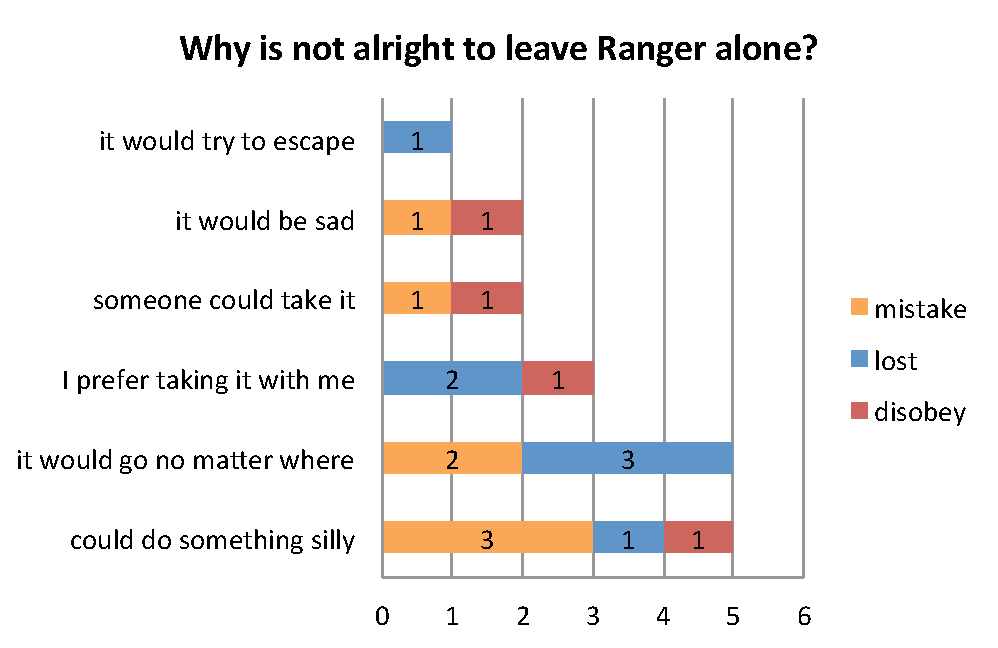
\includegraphics[width=0.9\linewidth]{domino-leave-why.pdf}
    \caption{\small Attributions of moral
        standing: we asked children whether it was alright to leave Ranger
        alone at home if they go on a 2-week vacation. Multiple answers
        (open-ended) were allowed when asked to justify their answer.}

    \label{fig:domino-leave-alone} 
\end{figure}		


\subsection{Manipulation check: Negligable impact of the conditions}

\subsection{Inter-subject and inter-group differences}

\subsection{Anthropomorphic projections and social engagement}

%%%%%%%%%%%%%%%%%%%%%%%%%%%%%%%%%%%%%%%%%%%%%%%%%%%%%%%%%%%%%%%%%%%%%%%%%%%%%%%%%%%%
%%%%%%%%%%%%%%%%%%%%%%%%%%%%%%%%%%%%%%%%%%%%%%%%%%%%%%%%%%%%%%%%%%%%%%%%%%%%%%%%%%%%
\section{Lessons Learned and Future Directions}

\begin{itemize}
\item It’s a challenge to interview young children ... 
\item Huge differences between the children and groups make it hard to draw general conclusions
\item Children did not perceive the 3 different conditions as we did not perceive the 3 different conditions as we expected
\item Coding scheme: “explore” category was not well defined
\end{itemize}




%%%%%%%%%%%%%%%%%%%%%%%%%%%%%%%%%%%%%%%%%%%%%%%%%%%%%%%%%%%%%%%%%%%%%%%%%%%%%%%%%%%%
%%%%%%%%%%%%%%%%%%%%%%%%%%%%%%%%%%%%%%%%%%%%%%%%%%%%%%%%%%%%%%%%%%%%%%%%%%%%%%%%%%%%
\section*{Acknowledgments}

This research was supported by the Swiss National Science Foundation through the
National Centre of Competence in Research Robotics.

%%%%%%%%%%%%%%%%%%%%%%%%%%%%%%%%%%%%%%%%%%%%%%%%%%%%%%%%%%%%%%%%%%%%%%%%%%%%%%%%%%%%
%%%%%%%%%%%%%%%%%%%%%%%%%%%%%%%%%%%%%%%%%%%%%%%%%%%%%%%%%%%%%%%%%%%%%%%%%%%%%%%%%%%%
\bibliographystyle{abbrv}
\bibliography{domino}

\balancecolumns

\end{document}
